\documentclass[12pt,reqno]{amsart}
\usepackage{/Users/johnmyers/GoogleDrive/tex/handout,/Users/johnmyers/GoogleDrive/tex/customcommands,polynom}
\usepackage{caption}

\hdr{MAT 240}{\S16.2 Iterated integrals}

\begin{document}

\textbf{Suggested problems:} 1-51 odd

\bigskip
\hrule

\bigskip

\prob Compute the following iterated integrals.

\begin{enumerate}
\item $\displaystyle\int_0^3 \int_0^4 (4x+3y) \ dx \ dy$ \vfill
\item $\displaystyle\int_0^2 \int_0^3 ( x^2+y^2) \ dy\ dx$ \vfill
\item $\displaystyle\int_0^1\int_0^1 ye^{xy} \ dx \ dy$ \vfill
\end{enumerate}

\prob A building is $8$ meters wide and $16$ meters long. It has a flat roof that is $12$ meters high at one corner, and $10$ meters high at each of the adjacent corners. What is the volume of the building?

\vfill
\newpage
\prob For each part below, write $\int_R f \ dA$ as an iterated integral of the shaded region $R$.

\begin{enumerate}
\item\textcolor{white}{blank}\\

\includegraphics[scale=1.25]{pic3.pdf}
\item\textcolor{white}{blank}\\

\includegraphics[scale=1.25]{pic4.pdf}
\item\textcolor{white}{blank}\\ 
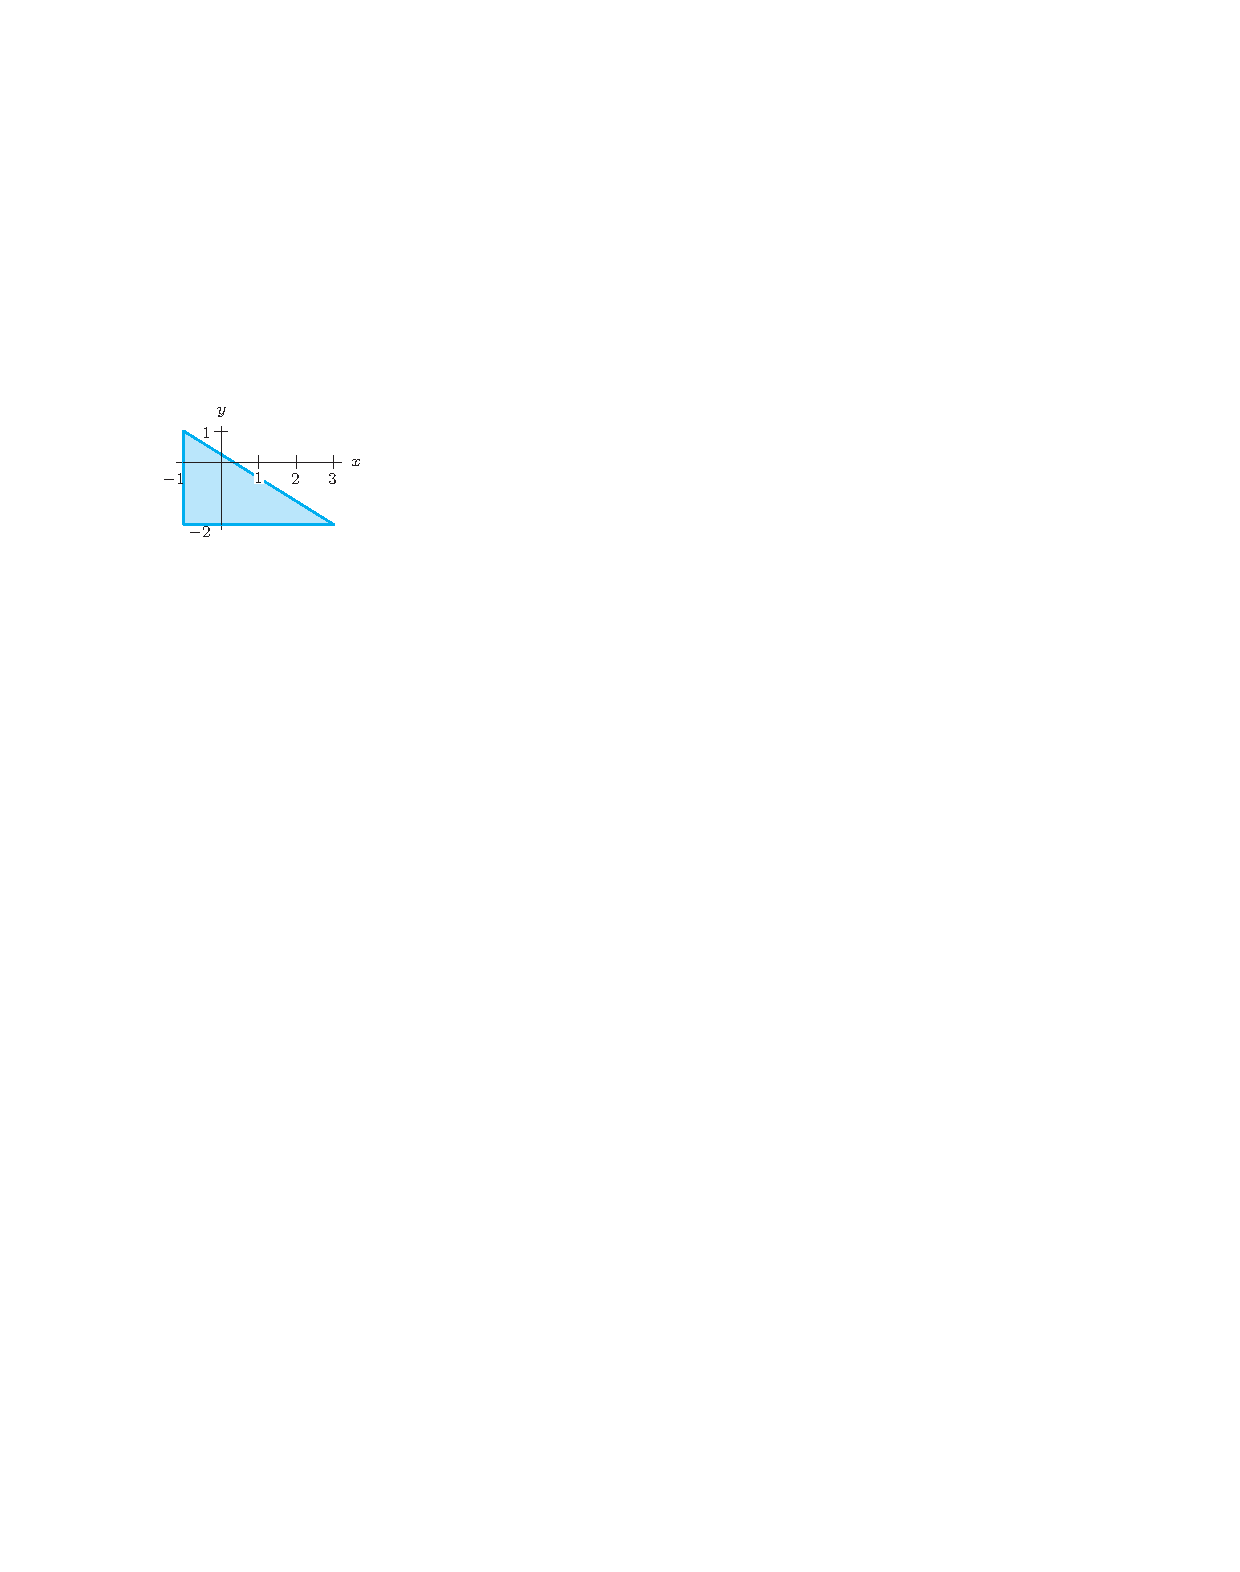
\includegraphics[scale=1.25]{pic5.pdf}
\end{enumerate}

\prob Compute the following iterated integrals. Sketch the region $R$ of integration.

\begin{enumerate}
\item $\displaystyle\int_0^2 \int_0^x e^{x^2} \ dy\ dx$\vfill
\item $\displaystyle\int_1^4 \int_{\sqrt{y}}^y x^2 y^3 \ dx \ dy$\vfill\newpage
\item $\displaystyle\int_1^5 \int_x^{2x} \sin{(x)} \ dy \ dx$
\end{enumerate}

\vfill
\prob Compute the following iterated integrals by reversing the order of integration.

\begin{enumerate}
\item $\displaystyle\int_0^2 \int_y^2 e^{x^2} \ dx \ dy$\vfill
\item $\displaystyle\int_0^1\int_{x^2}^1 \sqrt{y} \sin{(y)} \ dy dx$\vfill
\end{enumerate}


\end{document}